\documentclass{article}
\usepackage[left=0.75in,top=0.6in,right=0.75in,bottom=0.6in]{geometry} % Document margins
\usepackage{graphicx}

\title{Miaow - Implemented Instructions Specification}

\begin{document}
\maketitle
\section{Supported Instruction Formats}
\paragraph{}In this section the supported instruction formats are presented. A brief discription of each field is given. Refer to the ISA specification for more detailed information.
\subsection{SOPP}
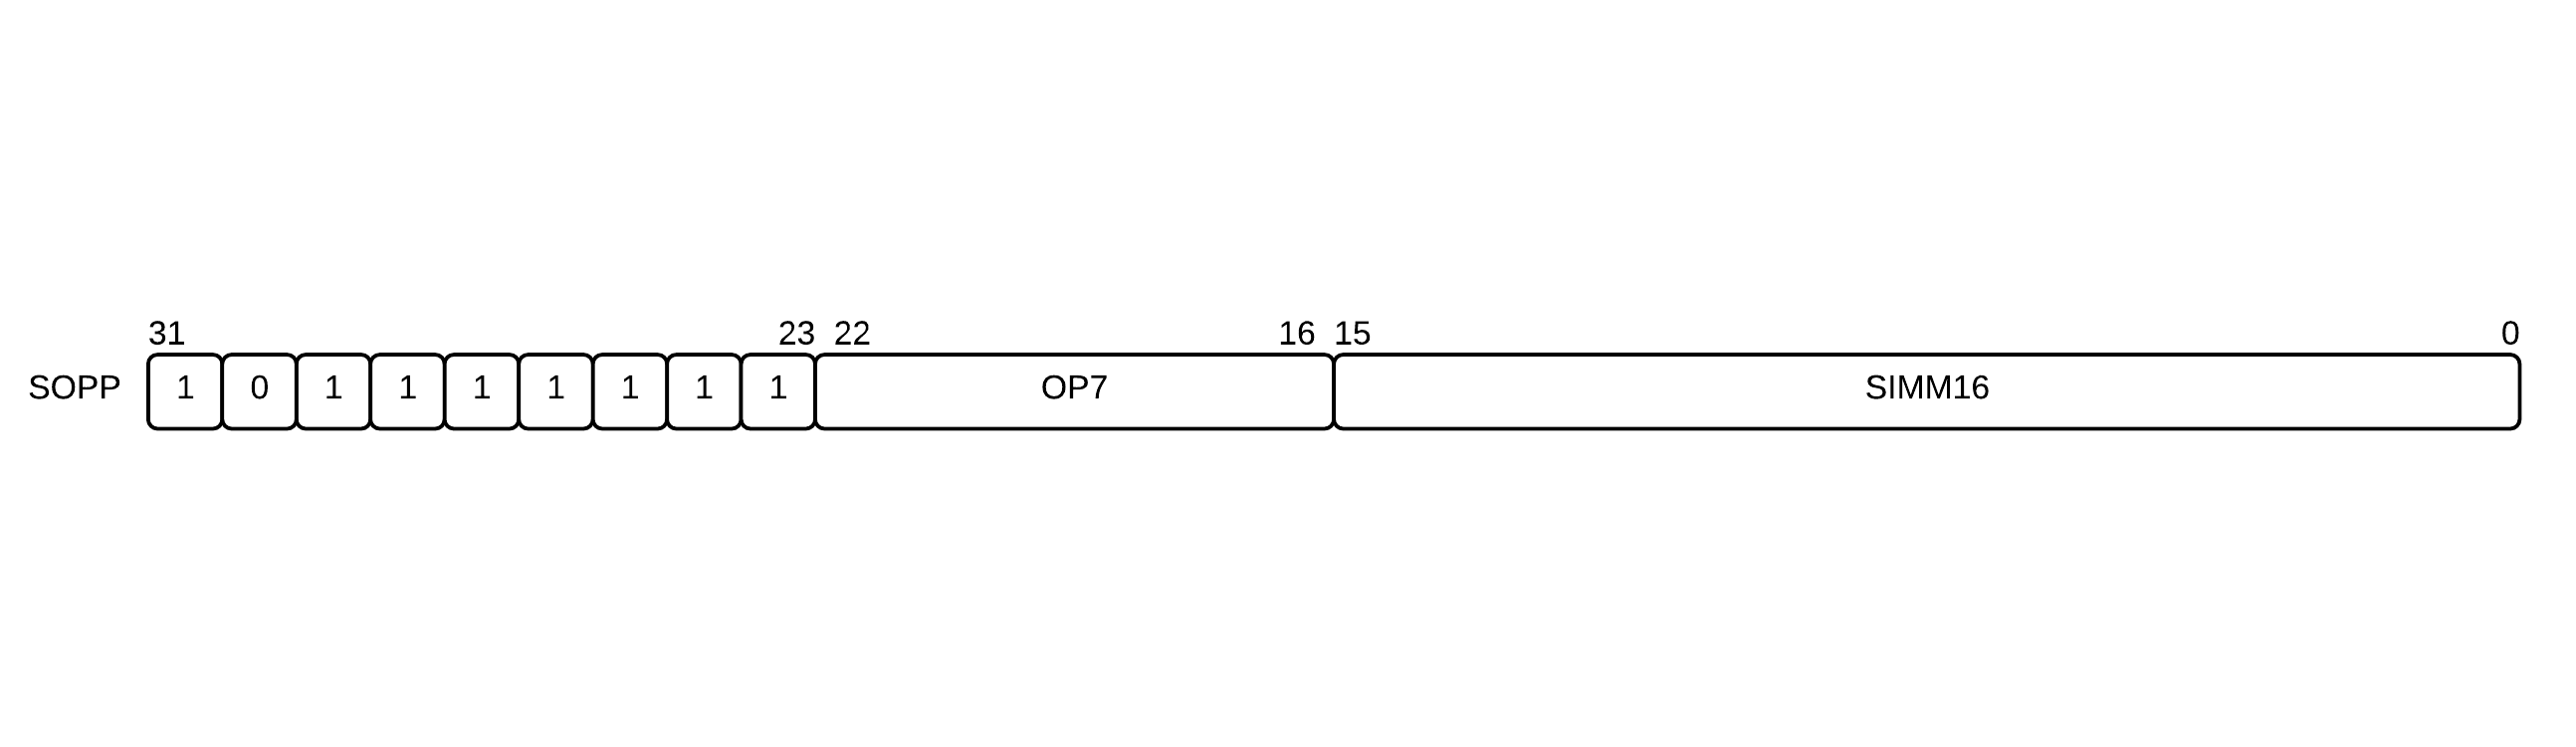
\includegraphics[width=7in, height=2in]{sopp.png} \\
\begin{description}
  \item [{OP[7]:}] Opcode for instruction.
  \item [{SIMM[16]:}] 16 bit immediate value. Signedness is determined by opcode.
\end{description}
\subsection{SOP1}
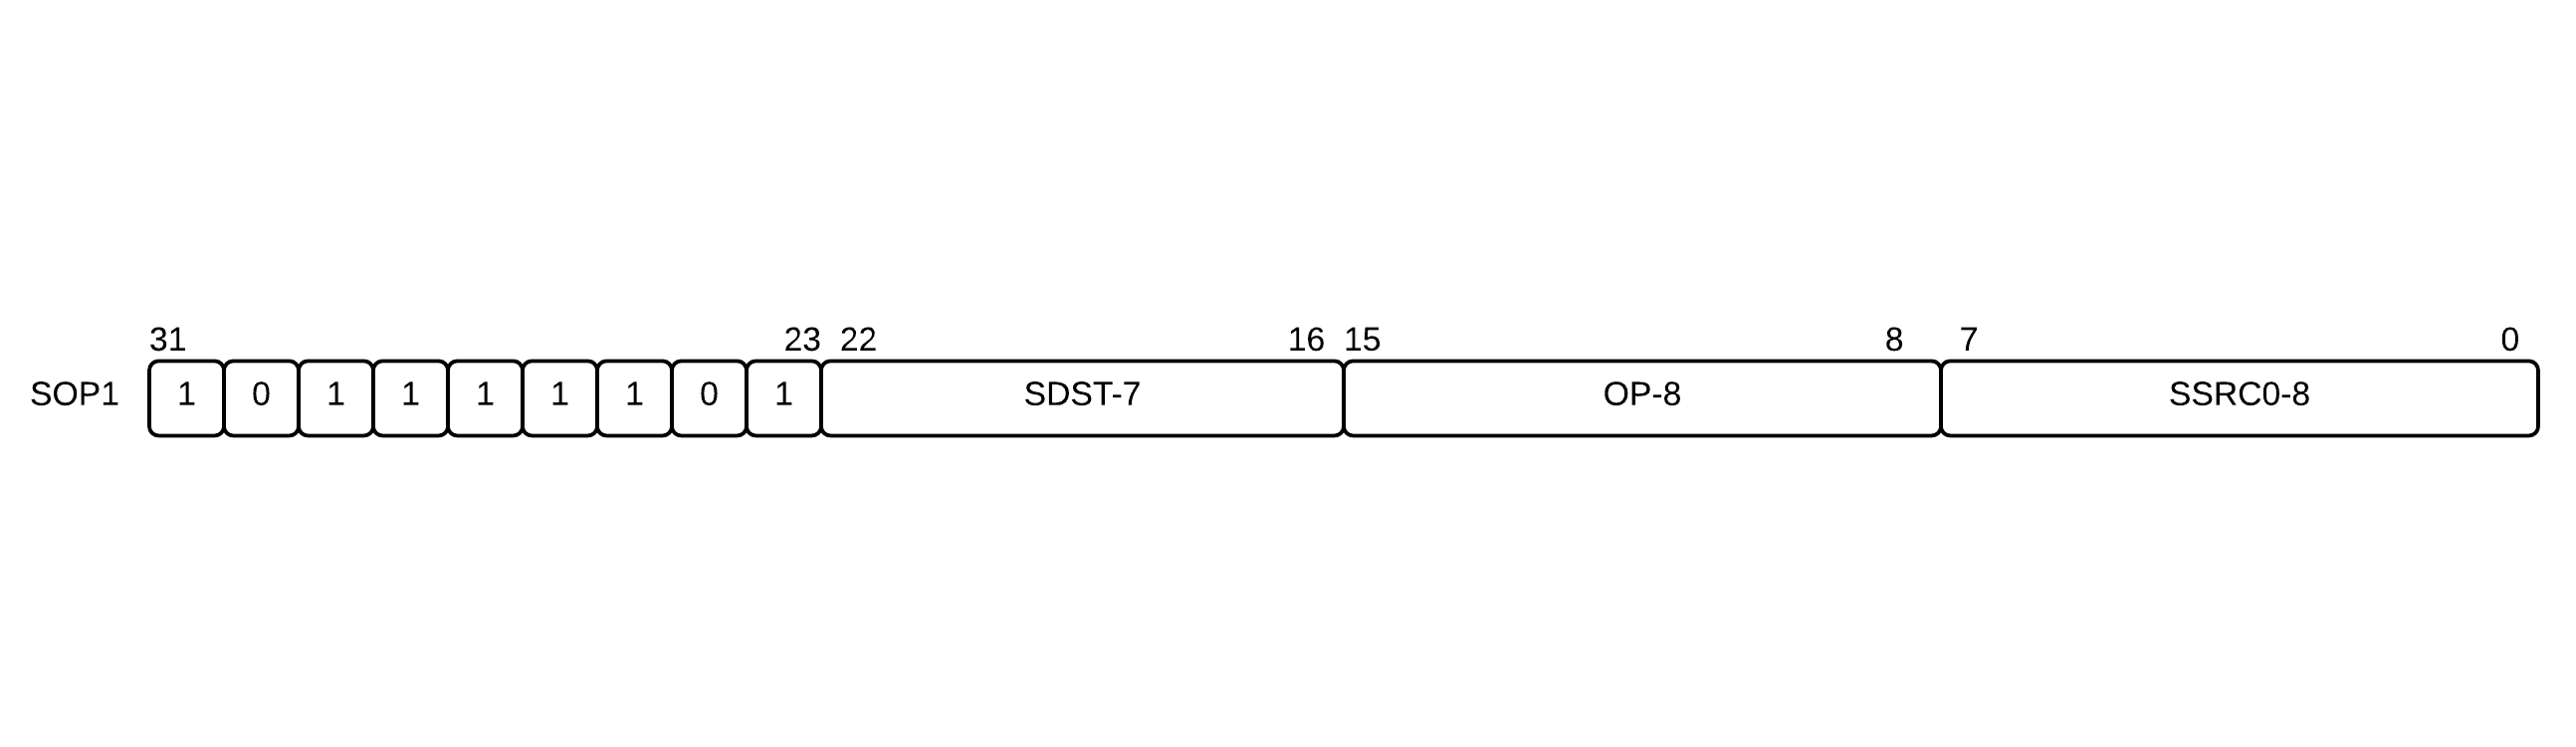
\includegraphics[width=7in, height=2in]{sop1.png} \\
\begin{description}
  \item [{OP[8]:}] Opcode for instruction.
  \item [{SDST[7]:}] Destination for the instruction. Must be a scalar 32 bit register. Can addres SGPRs, trap regisgers, VCC, M0 and EXEC.
  \item [{SSRC0[8]:}] Source of instruction. Must be a scalar 32 bit register. Support all values of SDST and some aditional constants.
\end{description}

\subsection{SOP2}
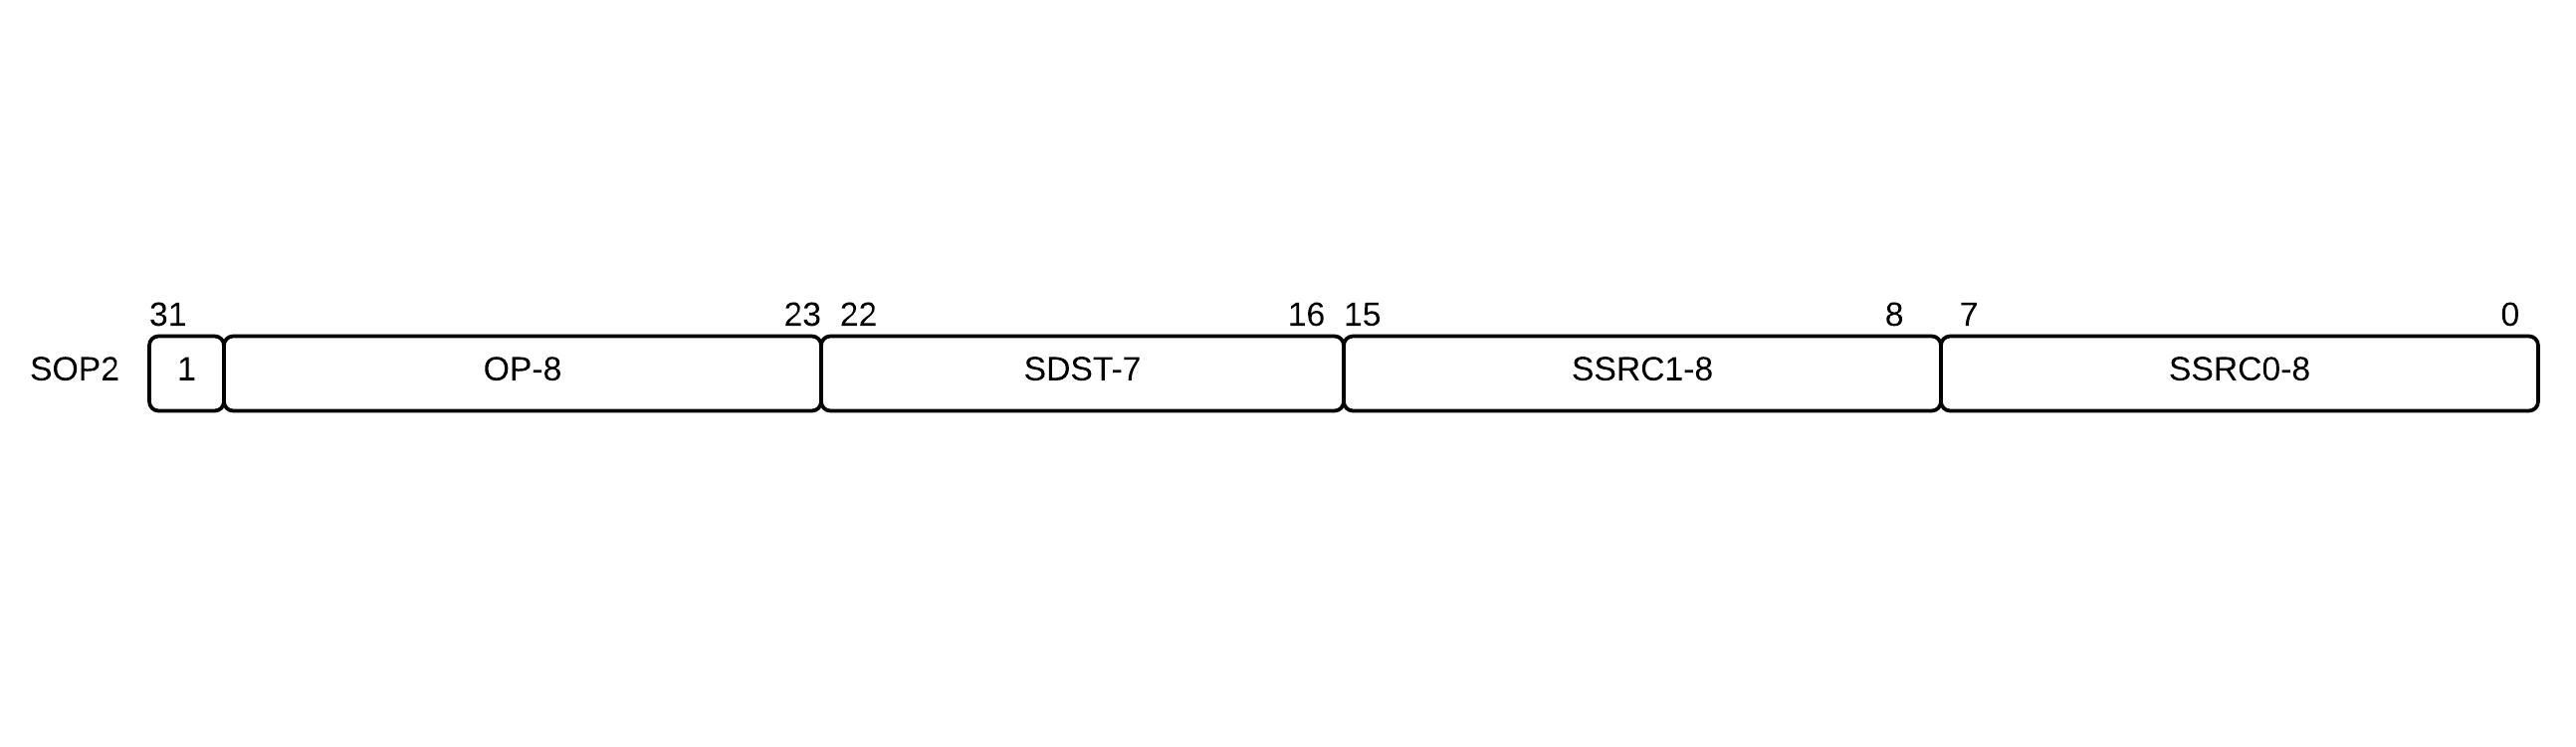
\includegraphics[width=7in, height=2in]{sop2.png} \\
\begin{description}
  \item [{OP[8]:}] Opcode for instruction.
  \item [{SDST[7]:}] Destination for the instruction. Must be a scalar 32 bit register. Can addres SGPRs, trap regisgers, VCC, M0 and EXEC.
  \item [{SSRC0[8]:}] Source of instruction. Must be a scalar 32 bit register. Support all values of SDST and some aditional constants.
  \item [{SSRC1[8]:}] Source of instruction. Must be a scalar 32 bit register. Support all values of SDST and some aditional constants.
\end{description}

\subsection{VOP1}
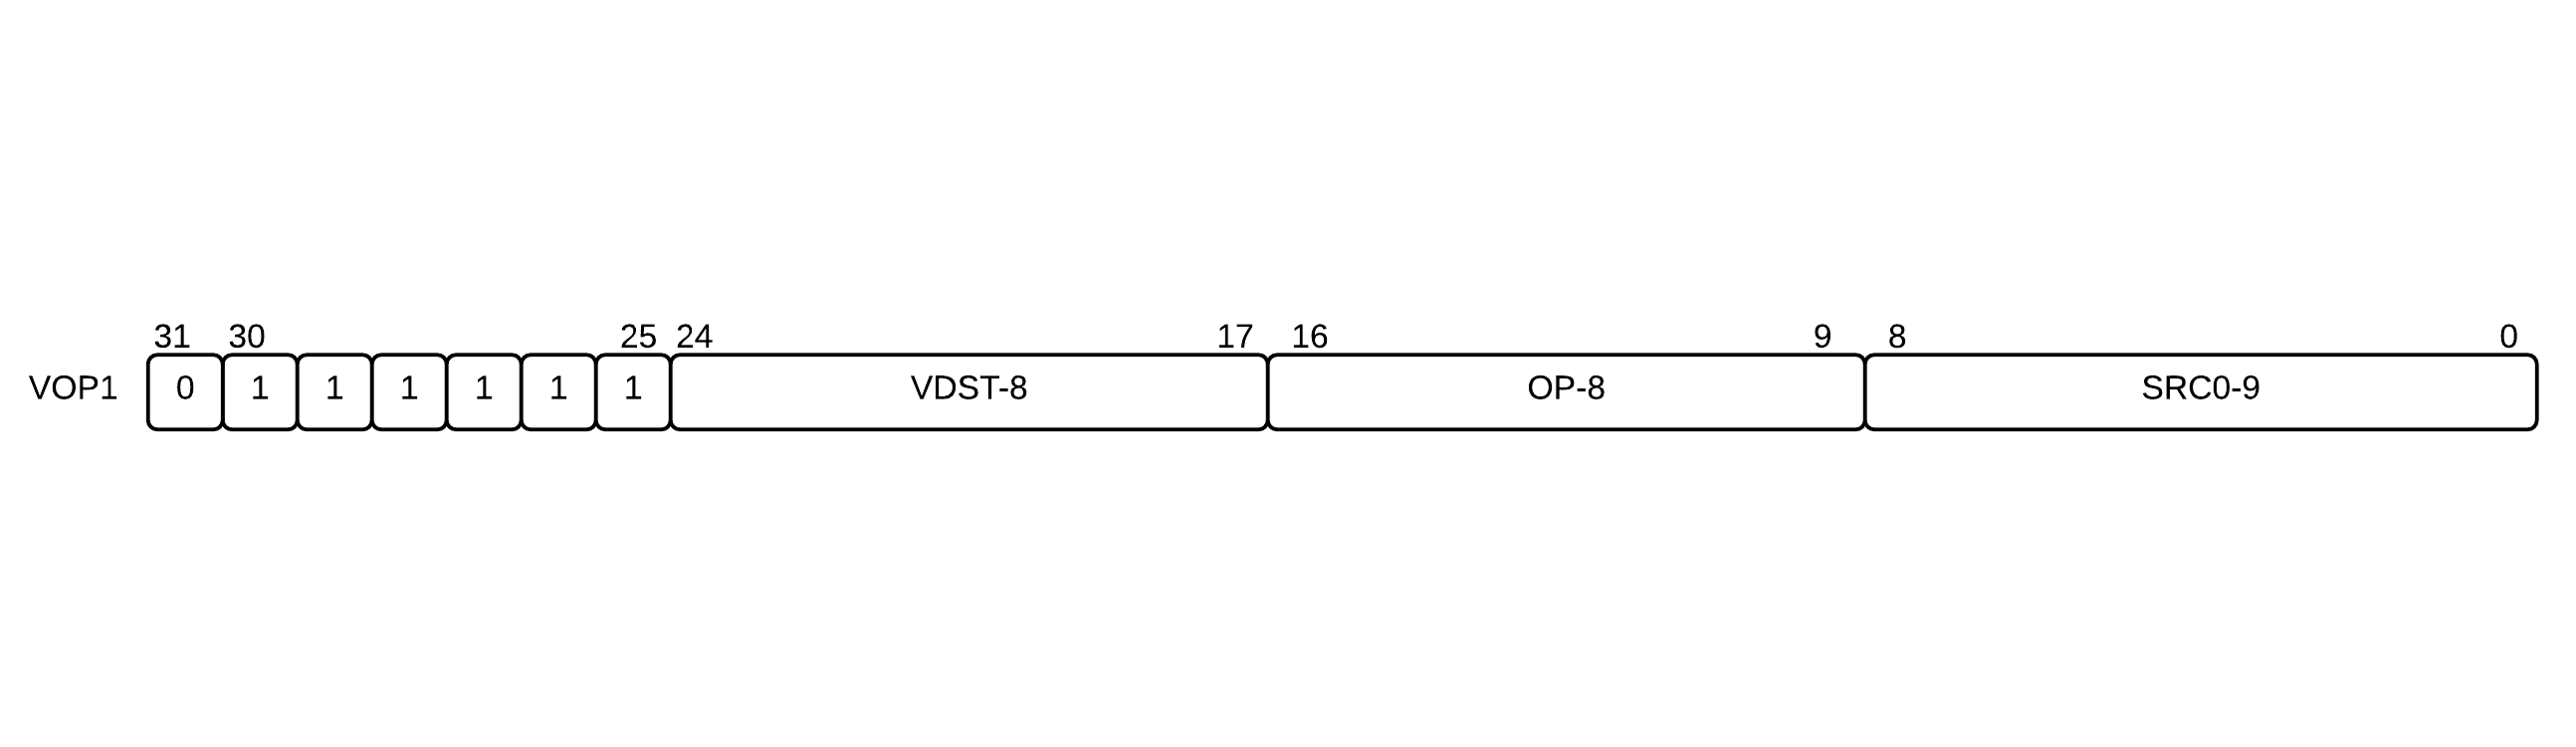
\includegraphics[width=7in, height=2in]{vop1.png} \\
\begin{description}
  \item [{OP[8]:}] Opcode for instruction.
  \item [{VDST[8]:}] Destination of the instruction. Can address all VGPRs.
  \item [{SRC0[9]:}] Source for the instruction. Can address all scalar values and VGPRs
\end{description}

\subsection{VOP2}
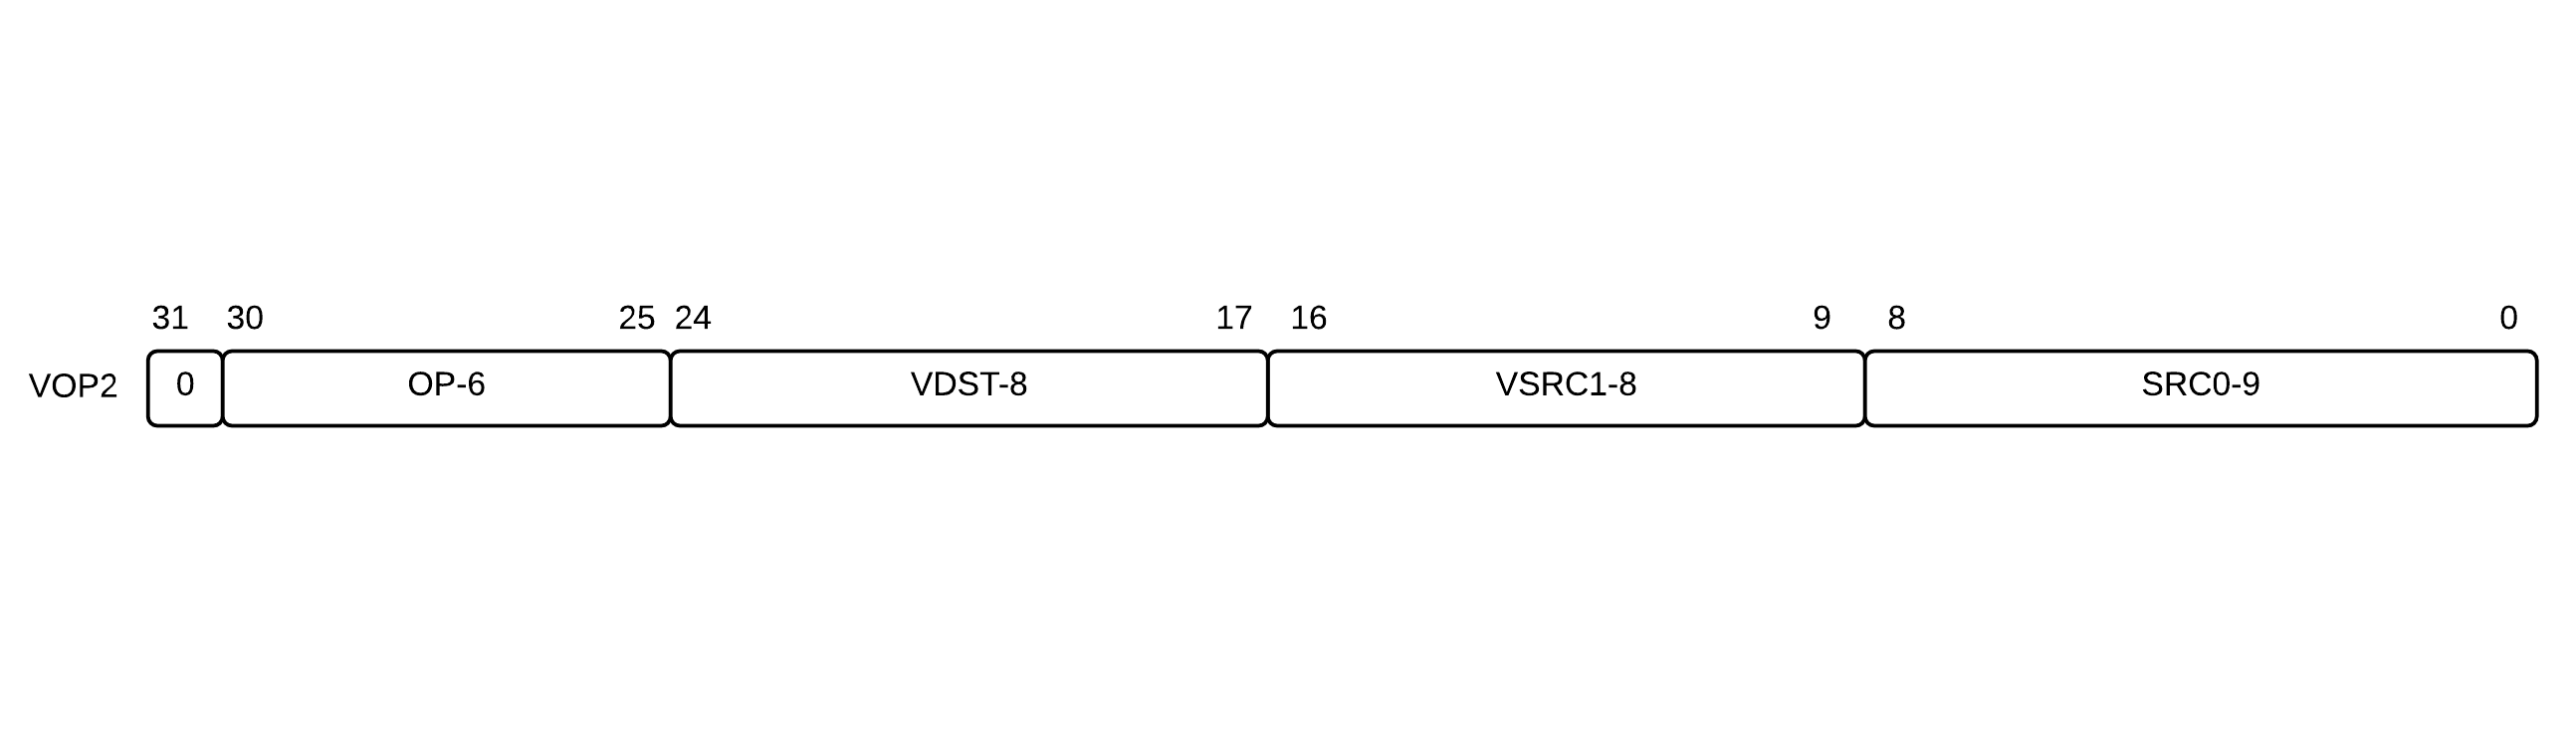
\includegraphics[width=7in, height=2in]{vop2.png} \\
\begin{description}
  \item [{OP[6]:}] Opcode for instruction.
  \item [{VDST[8]:}] Destination of the instruction. Can address all VGPRs.
  \item [{SRC0[9]:}] Source for the instruction. Can address all scalar values and VGPRs
  \item [{VSRC1[8]:}] Source for the instrucion. Can address all VGPRs
\end{description}

\subsection{SMRD}
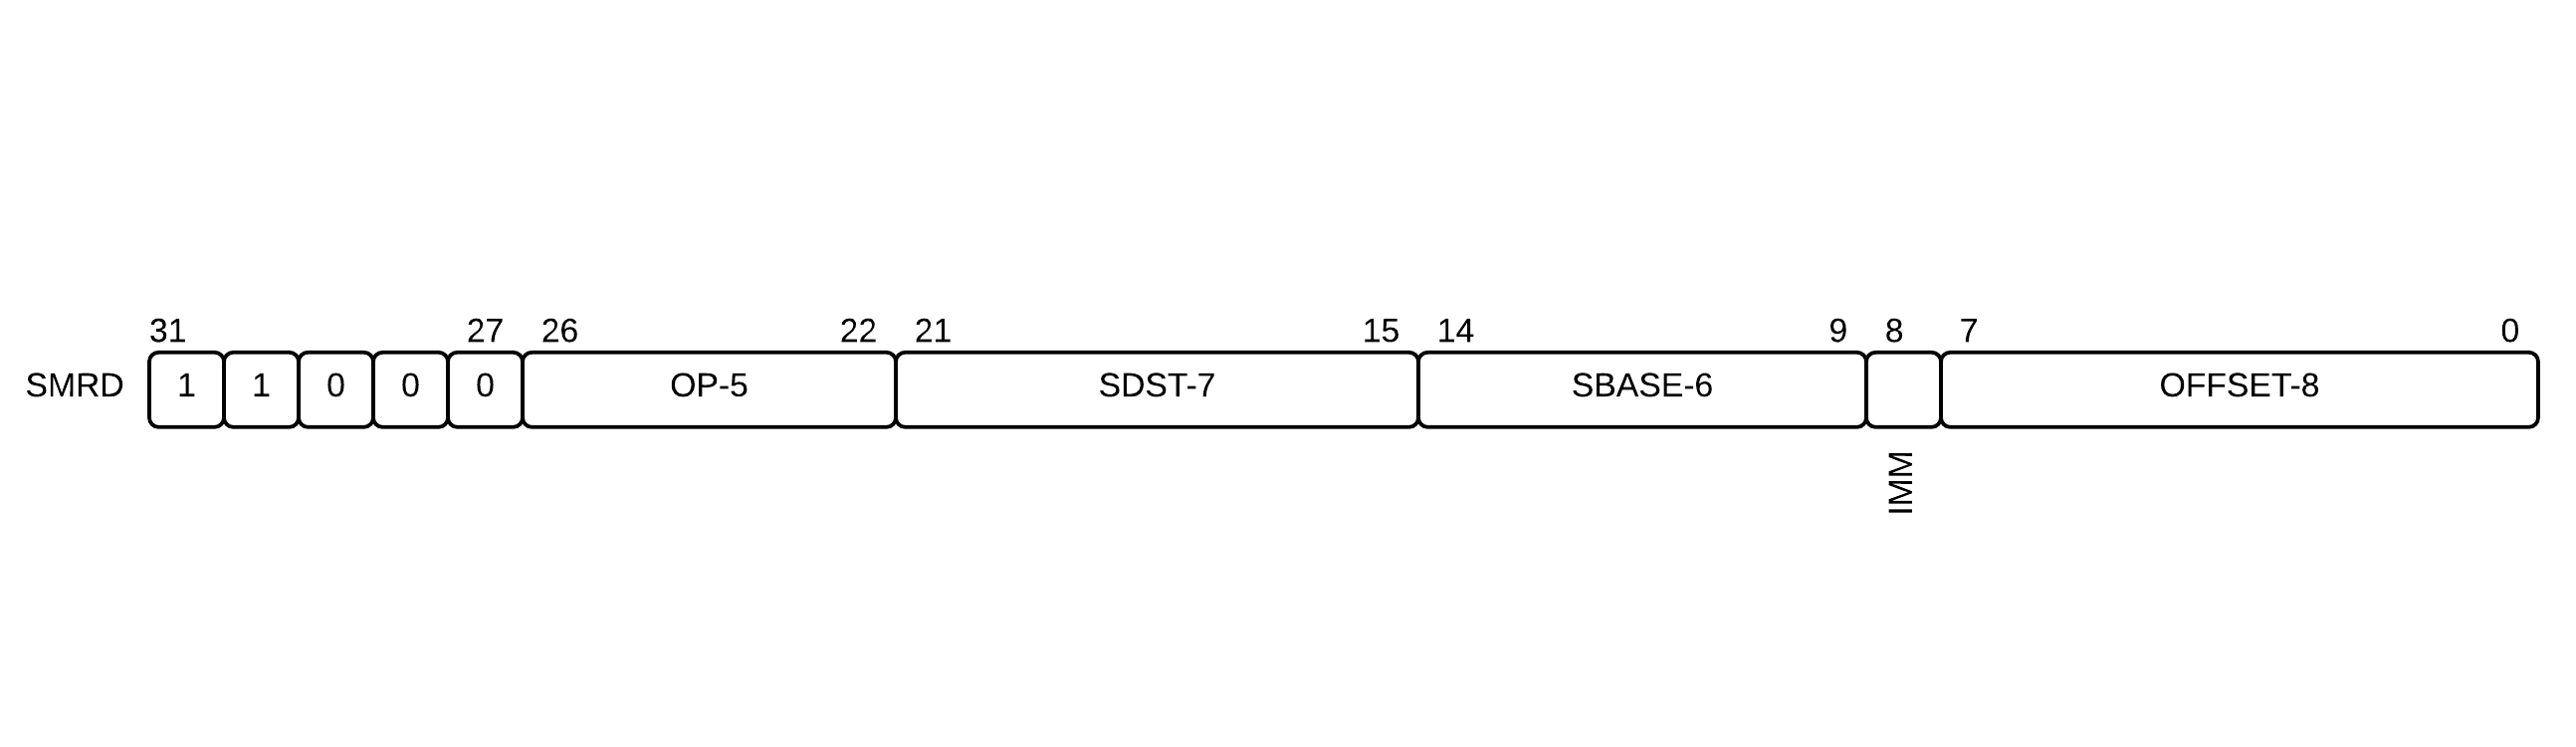
\includegraphics[width=7in, height=2in]{smrd.png} \\
\begin{description}
  \item [{OP[5]:}] Opcode for instruction.
  \item [{SDST[7]:}]  Destination for the instruction. Must be a scalar 32 bit register. Can addres SGPRs, trap regisgers, VCC, M0 and EXEC.
  \item [{SBASE[6]:}] Bits [6:1] of an aligned pair of SGPRs specifying {size[16], base[48]}, where base and size are in Dword units. The low-order bits are in the first SGPR.
  \item [{IMM[1]:}] If 1, OFFSET specifies a immediate offset, otherwise, offset specifies a sgpra that has the 8 bit offset.
  \item [{OFFSET[8]:}] 8 bits unsigned immediate to be added to SBASE or address to SGPR that has the 8 bit offset according to IMM flag
\end{description}

\subsection{MTBUF}
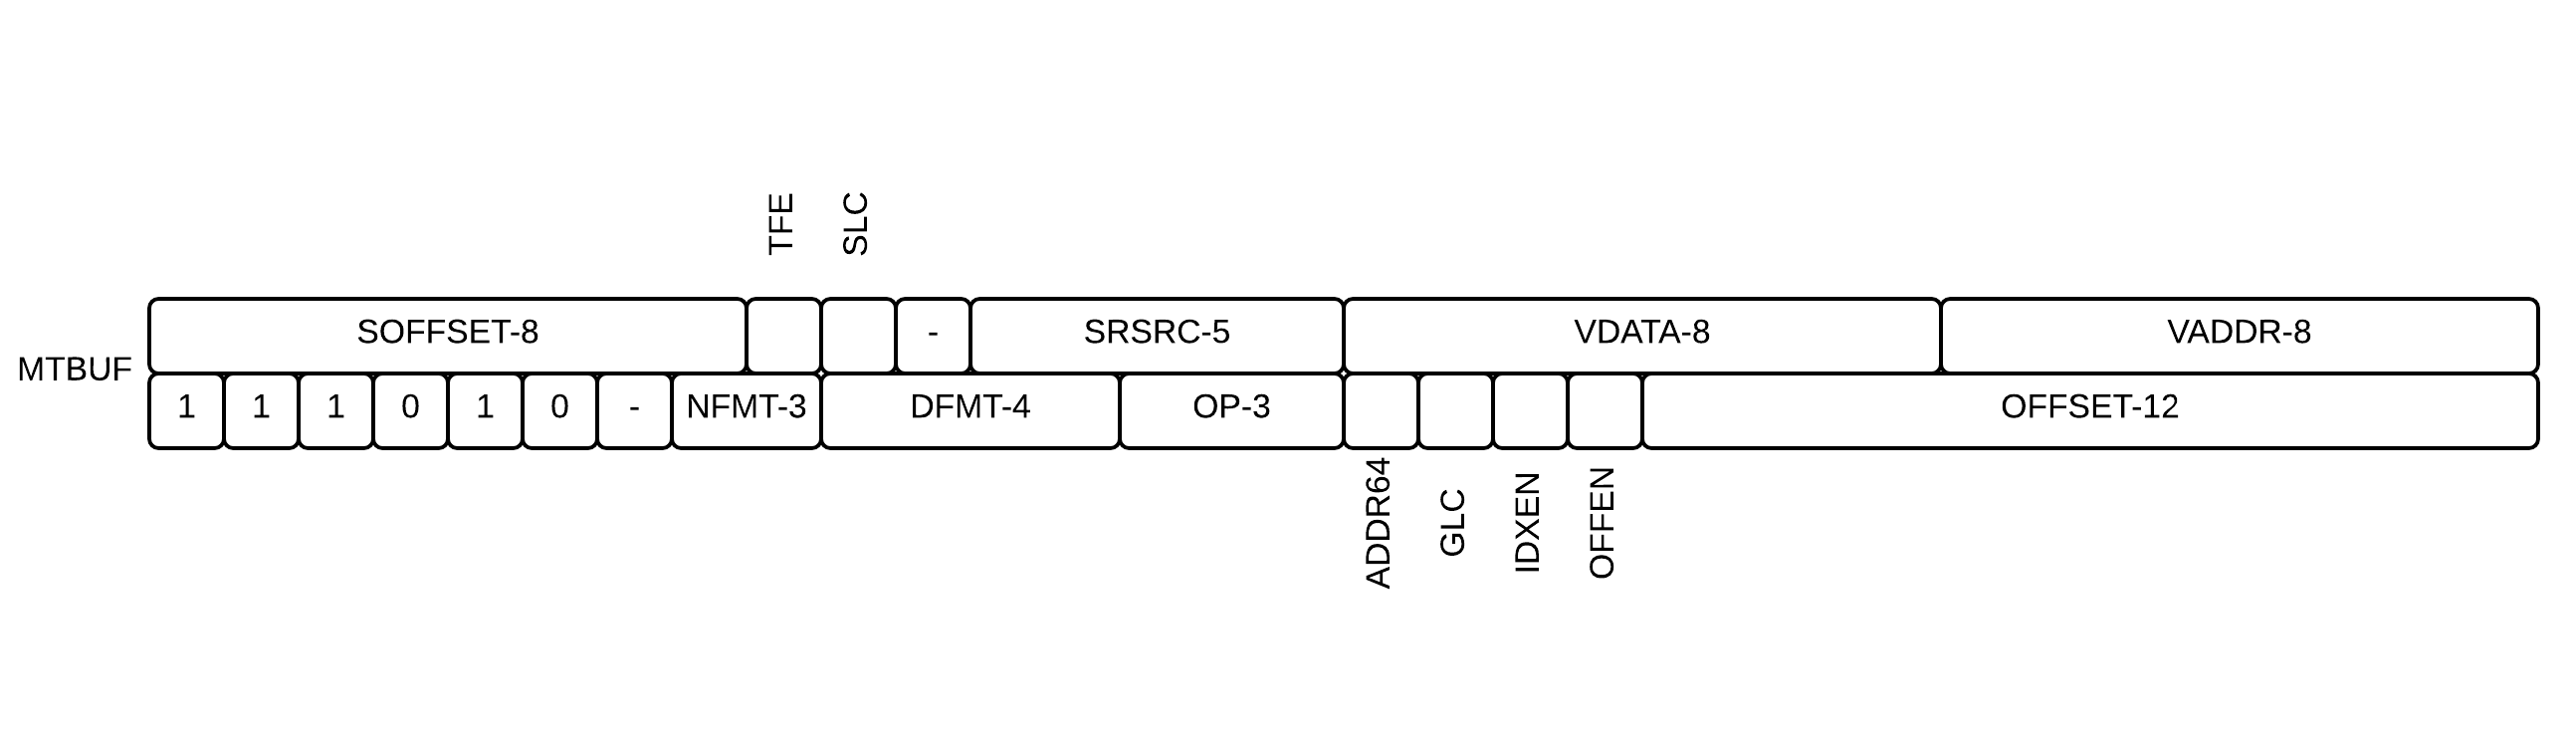
\includegraphics[width=7in, height=2in]{mtbuf.png} \\
\begin{description}
  \item[{OFFSET[12]:}] Unsigned bit offset for ADDR. Used only when offen is 0
  \item [{OFFEN[1]:}] If this is 0, offset is specified by OFFSET otherwise VADDR is an offset
  \item [{IDXEN[1]:}] If set, VADDR is an index otherwise index is 0.
  \item [{GLC[1]:}] If set, operation is globally coherent
  \item [{ADDR64[1]:}] If set, buffer addr is 64 bits.
  \item [{OP[3]:}] Opcode for instruction.
  \item [{DFMT[4]:}] Data format for typed buffer
  \item [{NFMT[3]:}] Number format for typed buffer
  \item [{VADDR[8]:}] Address for the operation. Can carry a offset or a index
  \item [{VDATA[8]:}] VGPR to read/write result to
  \item [{SRSRC[5]:}] ADDR of the 4 SGPRs that specify resource constant.
  \item [{SLC[1]:}] System level coherent
  \item [{TFE[1]:}] Texture fail enable
  \item [{SOFFSET[8]:}] Specifies the scalar offset to be added to memory addr.
\end{description}

\section{Instructions}
\subsection{Scalar ALU}
\begin{tabular}{l l l p{4.5in}}
Mnemonic & Format & Opcode & Discription \\ 
S\_ENDPGM & SOPP & 0x1 & Terminate wavefront. \\
S\_ADD\_U32/\_I32 & SOP2 & 0x0/0x2 & Unsigned or signed scalar add operation. SCC is set if carry out/overflow occurs. \\ 
S\_SUB\_I32 & SOP2 & 0x3 & Unsigned or signed scalar sub operation. SCC is set if carry out/overflow occurs. \\ 
S\_AND\_B32 & SOP2 & 0xE & Bitwise AND scalar operation. SCC is set if result is non-zero.\\
S\_OR\_B32 & SOP2 & 0x10 & Bitwise OR scalar operation. SCC is set if result is non-zero. \\
S\_MOV\_B32 & SOP1 & 0x3 & Move scalar source to scalar destination. \\
S\_NOT\_B32 & SOP1 & 0x7 & Bitwise NOT scalar operation. SCC is set if result is non-zero. \\
\end{tabular}

\subsection{Vector ALU}
\begin{tabular}{l l l p{4.5in}}
Mnemonic & Format & Opcode & Discription \\
V\_MOV\_B32 & VOP1 & 0x1 & Move vector value from source to vector destination. If a scalar source is given, the value is copied for each wave item. \\
V\_ADD\_I32 & VOP2 & 0x25 & \(D.u = S0.u + S1.u\)Integer signed/unsigned ADD. Carry out is written to VCC. If SRC0 is a scalar source, the value is copied for each wave item.  \\
V\_SUB\_I32 & VOP2 & 0x26 & \(D.u = S0.u - S1.u\) Integer sined/unsigned SUB. Borrow out is written to VCC. If SRC0 is a scalar source, the value is copied for each wave item. \\
V\_AND\_B32 & VOP2 & 0x1B & Logical bitwise AND. If SRC0 is a scalar source, the value is copied for each wave item.  \\
V\_OR\_B32 & VOP2 & 0x1C & Logical bitwise OR. If SRC0 is a scalar source, the value is copied for each wave item.  \\
V\_LSHLREV\_B32 & VOP2 & 0x1A & \(D.u = S1.u << S0.u[4:0]\). Scalar logical shift left. If SRC0 is a scalar source, the value iscopied for each wave item.  \\
V\_LSHRREV\_B32 & VOP2 & 0x16 & \(D.u = S1.u >> S0.u[4:0]\). Scalar logical shift right. If SRC0 is a scalar source, the value is copied for each wave item.\\
\end{tabular}

\subsection{Load store unit}
\subsubsection{S\_BUFFER\_LOAD}
\begin{description}
  \item[Format:] SMRD
  \item[Opcode:] 0x8
  \item[Discription:] Read a Dword from read-only buffer. 
  \begin{verbatim}
  m_offset = IMM ? OFFSET : SGPR[OFFSET]
  m_base = { SGPR[SBASE +1][15:0], SGPR[SBASE] }
  m_stride = SGPR[SBASE +1][31:16]
  m_num_records = SGPR[SBASE+2]
  m_size = (m_stride == 0) ? 1 : m_num_records
  m_addr = (SGPR[SBASE] + m_offset) & ~0x3
  SGPR[SDST] = read_dword_from_kcache(m_base, m_offset, m_size)
  \end{verbatim}
\end{description}
\subsubsection{T\_BUFFER\_LOAD\_FORMAT\_X}
\begin{description}
  \item[Format:] MTBUF
  \item[Opcode:] 0x00
  \item[Discription:] Typed load from buffer memory with format conversion. Addres is calculates according to:
  \begin{description}
    \item \begin{verbatim}
ADDR = Base + baseOffset + Ioffset + Voffset + Stride * (Vindex + TID)
       T#       SGPR        Instr     VGPR        T#    VGPR   0..63
    \end{verbatim}

    \item T\# is located at buffer resource constant, which in turn, is located at scalar registers addressed by SRSRC.
    \item See ISA spec, pag 8-9, table 8.5 for details. s
    \item Voffset is ignored when instruction bit “OFFEN”~==~0
    \item Vindex is ignored when instructino bit “IDXEN”~==~0
    \item TID is a constant value (0..63) unique to each thread in the wave. It is ignored when resource bit \\ADD\_TID\_ENABLE==0 
  \end{description}
\end{description}
\subsubsection{T\_BUFFER\_STORE\_FORMAT\_X}
\begin{description}
  \item[Format:] MTBUF
  \item[Opcode:] 0x04
  \item[Discription:] Typed store from buffer memory with format conversion. Address calculation is the same as \\T\_BUFFER\_LOAD\_FORMAT\_X
\end{description}

\section{Wishlist}
\begin{tabular}{l l l p{4.5in}}
Mnemonic & Format & Opcode & Discription \\
V\_CMP\_* & VOPC &  \\
S\_MIN\_U32 & SOP2 &  \\
S\_MAX\_U32 & SOP2 &  \\
\end{tabular}
\begin{itemize}
\item MULTIPLY 
\item WAITCNT 
\item MIAOW COMPILER!
\end{itemize}
\end{document}
